% ============================================================
\section{Introduction}
\label{sec:intro}
% ============================================================

Fine-tuning a time-series foundation model reshapes its internal
representations, and that reshaping is often read as forgetting: layer-wise CKA
drops are used to locate where forgetting happens~\citep{ramasesh2021anatomy},
representation similarity to predict how much a foundation model will
forget~\citep{mian2026frozen}, and feature distortion to explain why fine-tuning
underperforms out of distribution~\citep{kumar2022finetuning}.  The same reading
motivates freezing the encoder, regularising toward the pre-trained
weights~\citep{li2018l2sp, kirkpatrick2017ewc}, and low-rank adapters, which
time-series work adopts partly to retain the pre-trained
representation~\citep{gupta2024lowrank, laglil2026foundation} (and partly for
efficiency or against overfitting).  Insofar as they protect the representation,
those prescriptions presuppose that it was worth preserving \emph{on the target
task}.

Whether a change was harmful is an interventional question: fine-tune the whole
model, fine-tune it again with the encoder frozen on the same data and budget, and
compare the two on windows neither run selected on.  That costs one extra training
run, so we do not offer CKA as a cheaper stand-in for it.  We ask the converse:
when an analysis reads a CKA drop as evidence of forgetting, is that reading
warranted for time-series foundation models?  Tested against the intervention, it
is not.

\textbf{One checkpoint, two datasets, opposite lessons.}  Fine-tune Moirai-Base
on ETTh1 and its encoder barely moves (CKA $0.755$ against the pre-trained
encoder), and the model ends $22.8\%$ \emph{worse} than not fine-tuning at all.
Fine-tune the same checkpoint on ETTh2 and the encoder restructures far more, to
CKA $0.460$, and the model ends $31.4\%$ \emph{better}.  Read drift as damage and
you would have protected the run that needed no protection and left alone the one
that did.

\begin{figure}[t]
\centering
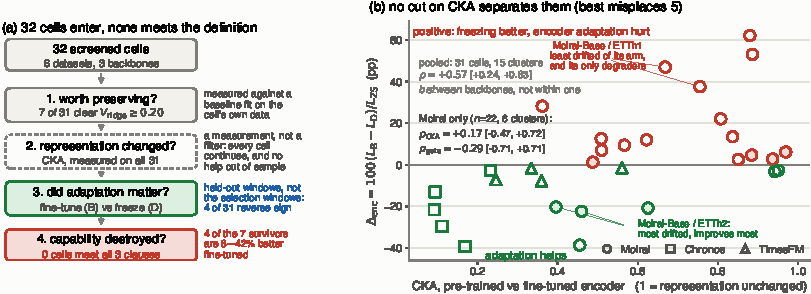
\includegraphics[width=\linewidth]{fig1_diagnostic_flow.pdf}
\caption{\textbf{(a)}~The screen of \S\ref{sec:method} over the 31 cells that
carry a selection-split gate: CKA filters none of them, and no cell meets the
degradation definition.  \textbf{(b)}~The same cells as CKA against held-out
$\denc$ (positive ${=}$ freezing better): no cut on CKA separates the cells
adaptation helped from the cells it hurt.  The labelled pairs are the running
example: Moirai-Base's two \emph{least} drifted cells are its only two that
degrade, and its two most drifted improve the most (\S\ref{sec:exp3}).  Filled
markers clear the gate; both $\rho$ are clustered by backbone${\times}$dataset,
and only Moirai has enough cells to estimate one within a backbone
(Appendix~\ref{app:clustered}).}
\label{fig:screen}
\end{figure}

\textbf{What we test, and on what.}  We screen \textbf{32 cells}: three backbones
(Moirai Small 13.8M, Base 91M, Large 311M; Chronos-T5~\citep{ansari2024chronos};
TimesFM-2.5~\citep{das2024timeseries}, with MOMENT~\citep{goswami2024moment}
screened and excluded), six datasets and two forecast horizons.  Each cell pairs
a full fine-tune with a frozen-encoder run, and on the Moirai cells with a strict
freeze under which nothing upstream of the forecasting head can move, at 3--10
seeds.  We then ask four questions in order (Figure~\ref{fig:screen}a).  Is
there a pre-trained capability worth preserving (\S\ref{sec:forecasting})?  Does
letting the encoder adapt help or hurt (\S\ref{sec:exp2})?  Does CKA order the
answer (\S\ref{sec:exp3})?  And where damage is forced, or looked for on other
datasets, does CKA see it (\S\ref{sec:exp4})?  Every claim is about the
checkpoints, datasets and protocols we evaluated; the readings we decline are
listed under \emph{Scope of the claims} in the Ethics Statement.

\textbf{Contributions.}
\begin{enumerate}\itemsep1pt
  \item \textbf{Drift does not track the intervention.}  Within Moirai-Base the
    least drifted cells are the only ones that degrade; a pre-registered positive
    control drives CKA on the original task's inputs to $0.063$ while that task
    \emph{improves} by $23.3\%$; and \pending{out-of-domain retention result}.
    Across cells, within Moirai, the only backbone with enough cells to ask,
    $\rho{=}{+}0.168$ (clustered CI $[-0.469,{+}0.717]$): an interval that rules out
    a strong positive association but not a moderate one, so we claim no ordering
    rather than the absence of one.  Out of sample, adding CKA to backbone and
    protocol lowers leave-one-cluster-out $R^2$ from $+0.201$ to $+0.176$
    (\S\ref{sec:exp3}).
  \item \textbf{Two measurement prerequisites for any such comparison.}  Scoring
    the frozen-encoder comparison on the windows it was selected on reverses its
    sign on 4 of 31 cells, all toward flattering the frozen encoder; and an unfitted
    linear baseline would move 17 of Moirai's 21 cells across the capability screen.
    With both in place, \textbf{only 7 of the 31 scored cells} show a pre-trained
    advantage over a linear regression fit on the target data, all of them Moirai
    on ETTh2 and ETTm2 (\S\S\ref{sec:method},~\ref{sec:forecasting}).
  \item \textbf{No harmful encoder adaptation under a prespecified definition.}
    On multiplicity-adjusted paired intervals the 31 cells split 2 freezing-better,
    4 adaptation-better and 25 inconclusive, and both freezing-better cells are
    ones the screen rejects; on five of the seven that pass it, full fine-tuning
    improves on zero-shot (\S\ref{sec:exp2}).
\end{enumerate}
